% 保留原始面板、实拍、示例与全部连线；仅以 TikZ 覆盖说明标签。
\begin{tikzpicture}
\node[anchor=south west,inner sep=0] (im) at (0,0) {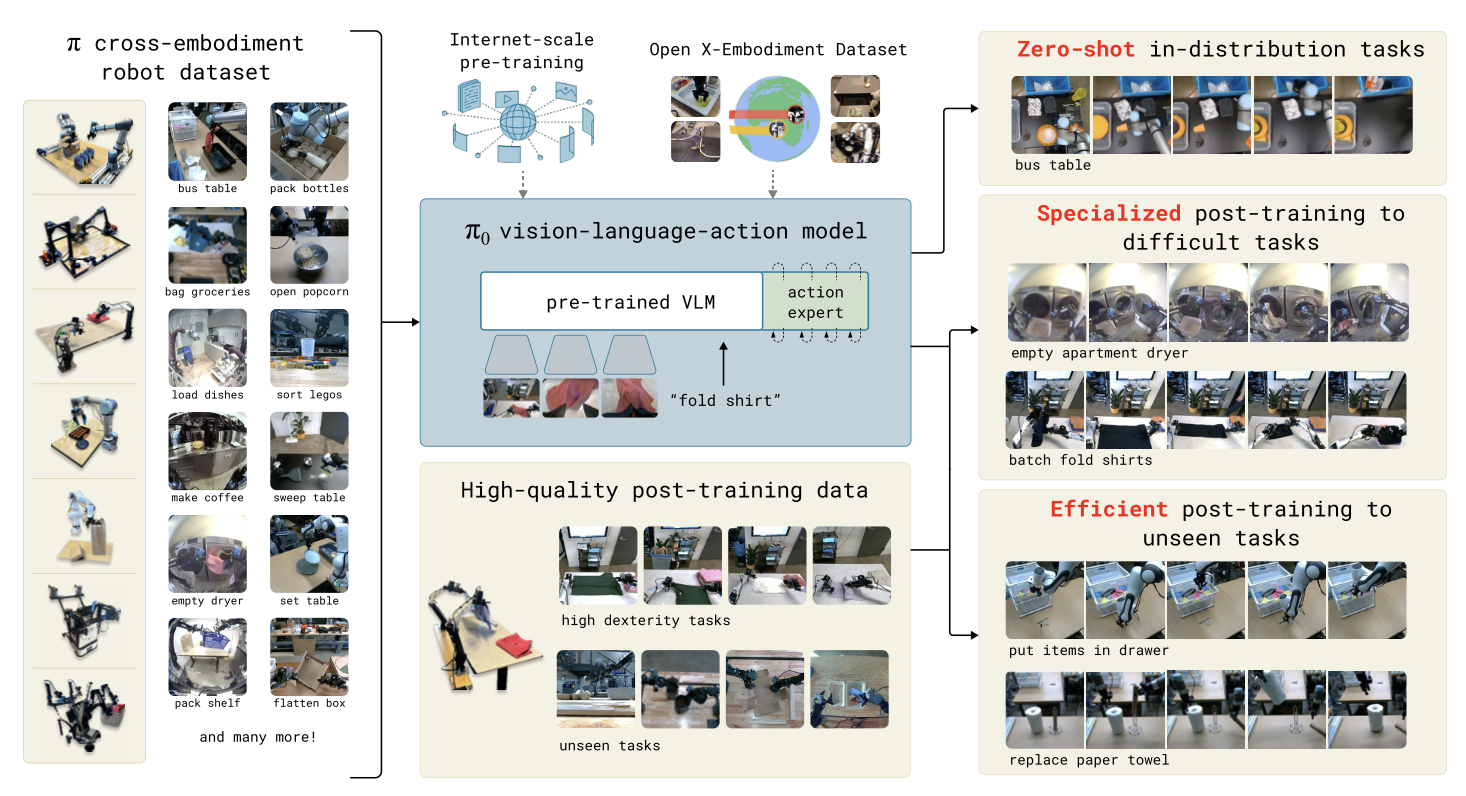
\includegraphics[width=\linewidth]{figures/pizero.png}};
\begin{scope}[x={(im.south east)},y={(im.north west)}]
\fill[white] (0.045703,0.896985) rectangle (0.223056,0.964824);
\node[align=center,inner sep=0pt,font=\fontsize{9}{10}\selectfont,text width=0.177353\linewidth,rotate=0] at (0.134379,0.930905) {$\pi$ 跨具身\\机器人数据集};
\fill[white] (0.304911,0.907035) rectangle (0.415416,0.966080);
\node[align=center,inner sep=0pt,font=\fontsize{8}{9}\selectfont,text width=0.110505\linewidth,rotate=0] at (0.360164,0.936558) {互联网规模\\预训练};
\fill[white] (0.440655,0.922111) rectangle (0.622101,0.954774);
\node[align=center,inner sep=0pt,font=\fontsize{8}{9}\selectfont,text width=0.181446\linewidth,rotate=0] at (0.531378,0.938442) {Open X-Embodiment 数据集};
\fill[blue!12] (0.314461,0.689698) rectangle (0.596180,0.728643);
\node[align=center,inner sep=0pt,font=\fontsize{9}{10}\selectfont,text width=0.281719\linewidth,rotate=0] at (0.455321,0.709171) {$\pi_0$ 视觉语言动作模型};
\fill[white] (0.331514,0.587940) rectangle (0.516371,0.655779);
\node[align=center,inner sep=0pt,font=\fontsize{8}{9}\selectfont,text width=0.184857\linewidth,rotate=0] at (0.423943,0.621859) {预训练视觉语言模型};
\fill[green!15] (0.524557,0.587940) rectangle (0.590723,0.655779);
\node[align=center,inner sep=0pt,font=\fontsize{7.2}{8.2}\selectfont,text width=0.066166\linewidth,rotate=0] at (0.557640,0.621859) {动作\\专家};
\fill[blue!12] (0.452251,0.476131) rectangle (0.553206,0.512563);
\node[align=center,inner sep=0pt,font=\fontsize{7.2}{8.2}\selectfont,text width=0.100955\linewidth,rotate=0] at (0.502729,0.494347) {“折叠衬衫”};
\fill[white] (0.309686,0.365578) rectangle (0.607776,0.402010);
\node[align=center,inner sep=0pt,font=\fontsize{9}{10}\selectfont,text width=0.298090\linewidth,rotate=0] at (0.458731,0.383794) {高质量后训练数据};
\fill[white] (0.384038,0.201005) rectangle (0.584584,0.231156);
\node[align=center,inner sep=0pt,font=\fontsize{8}{9}\selectfont,text width=0.200546\linewidth,rotate=0] at (0.484311,0.216080) {高灵巧度任务};
\fill[white] (0.379945,0.047739) rectangle (0.513643,0.075377);
\node[align=center,inner sep=0pt,font=\fontsize{8}{9}\selectfont,text width=0.133697\linewidth,rotate=0] at (0.446794,0.061558) {未见过的任务};
\fill[white] (0.687585,0.920854) rectangle (0.979536,0.953518);
\node[align=center,inner sep=0pt,font=\fontsize{9}{10}\selectfont,text width=0.291951\linewidth,rotate=0] at (0.833561,0.937186) {分布内任务的零样本表现};
\fill[white] (0.703274,0.776382) rectangle (0.772851,0.802764);
\node[align=center,inner sep=0pt,font=\fontsize{7.5}{8.5}\selectfont,text width=0.069577\linewidth,rotate=0] at (0.738063,0.789573) {收拾餐桌};
\fill[white] (0.685539,0.683417) rectangle (0.980900,0.747487);
\node[align=center,inner sep=0pt,font=\fontsize{9}{10}\selectfont,text width=0.295362\linewidth,rotate=0] at (0.833220,0.715452) {通过专门后训练\\完成困难任务};
\fill[white] (0.688267,0.542714) rectangle (0.843111,0.567839);
\node[align=center,inner sep=0pt,font=\fontsize{7.5}{8.5}\selectfont,text width=0.154843\linewidth,rotate=0] at (0.765689,0.555276) {清空公寓中的烘干机};
\fill[white] (0.685539,0.407035) rectangle (0.850614,0.434673);
\node[align=center,inner sep=0pt,font=\fontsize{7.5}{8.5}\selectfont,text width=0.165075\linewidth,rotate=0] at (0.768076,0.420854) {批量折叠衬衫};
\fill[white] (0.684857,0.309045) rectangle (0.978854,0.374372);
\node[align=center,inner sep=0pt,font=\fontsize{9}{10}\selectfont,text width=0.293997\linewidth,rotate=0] at (0.831855,0.341709) {通过高效后训练\\完成未见过的任务};
\fill[white] (0.685539,0.163317) rectangle (0.850614,0.193467);
\node[align=center,inner sep=0pt,font=\fontsize{7.5}{8.5}\selectfont,text width=0.165075\linewidth,rotate=0] at (0.768076,0.178392) {把物品放入抽屉};
\fill[white] (0.685539,0.026382) rectangle (0.854025,0.055276);
\node[align=center,inner sep=0pt,font=\fontsize{7.5}{8.5}\selectfont,text width=0.168486\linewidth,rotate=0] at (0.769782,0.040829) {更换厨房纸卷};
\fill[white] (0.131651,0.057789) rectangle (0.228513,0.085427);
\node[align=center,inner sep=0pt,font=\fontsize{8}{9}\selectfont,text width=0.096862\linewidth,rotate=0] at (0.180082,0.071608) {还有更多！};
\fill[white] (0.107776,0.747487) rectangle (0.173943,0.776382);
\node[align=center,inner sep=0pt,font=\fontsize{6.2}{7.2}\selectfont,text width=0.066166\linewidth,rotate=0] at (0.140859,0.761935) {收餐桌};
\fill[white] (0.177353,0.747487) rectangle (0.243520,0.776382);
\node[align=center,inner sep=0pt,font=\fontsize{6.2}{7.2}\selectfont,text width=0.066166\linewidth,rotate=0] at (0.210437,0.761935) {装瓶};
\fill[white] (0.107776,0.615578) rectangle (0.173943,0.644472);
\node[align=center,inner sep=0pt,font=\fontsize{6.2}{7.2}\selectfont,text width=0.066166\linewidth,rotate=0] at (0.140859,0.630025) {杂货装袋};
\fill[white] (0.177353,0.615578) rectangle (0.243520,0.644472);
\node[align=center,inner sep=0pt,font=\fontsize{6.2}{7.2}\selectfont,text width=0.066166\linewidth,rotate=0] at (0.210437,0.630025) {开爆米花};
\fill[white] (0.107776,0.483668) rectangle (0.173943,0.512563);
\node[align=center,inner sep=0pt,font=\fontsize{6.2}{7.2}\selectfont,text width=0.066166\linewidth,rotate=0] at (0.140859,0.498116) {装餐具};
\fill[white] (0.177353,0.483668) rectangle (0.243520,0.512563);
\node[align=center,inner sep=0pt,font=\fontsize{6.2}{7.2}\selectfont,text width=0.066166\linewidth,rotate=0] at (0.210437,0.498116) {理乐高};
\fill[white] (0.107776,0.351759) rectangle (0.173943,0.380653);
\node[align=center,inner sep=0pt,font=\fontsize{6.2}{7.2}\selectfont,text width=0.066166\linewidth,rotate=0] at (0.140859,0.366206) {煮咖啡};
\fill[white] (0.177353,0.351759) rectangle (0.243520,0.380653);
\node[align=center,inner sep=0pt,font=\fontsize{6.2}{7.2}\selectfont,text width=0.066166\linewidth,rotate=0] at (0.210437,0.366206) {扫桌面};
\fill[white] (0.107776,0.221106) rectangle (0.173943,0.250000);
\node[align=center,inner sep=0pt,font=\fontsize{6.2}{7.2}\selectfont,text width=0.066166\linewidth,rotate=0] at (0.140859,0.235553) {清烘干机};
\fill[white] (0.177353,0.221106) rectangle (0.243520,0.250000);
\node[align=center,inner sep=0pt,font=\fontsize{6.2}{7.2}\selectfont,text width=0.066166\linewidth,rotate=0] at (0.210437,0.235553) {摆餐桌};
\fill[white] (0.107776,0.089196) rectangle (0.173943,0.118090);
\node[align=center,inner sep=0pt,font=\fontsize{6.2}{7.2}\selectfont,text width=0.066166\linewidth,rotate=0] at (0.140859,0.103643) {整理货架};
\fill[white] (0.177353,0.089196) rectangle (0.243520,0.118090);
\node[align=center,inner sep=0pt,font=\fontsize{6.2}{7.2}\selectfont,text width=0.066166\linewidth,rotate=0] at (0.210437,0.103643) {压平盒子};
\end{scope}
\end{tikzpicture}
